\documentclass[12pt,a4paper,english]{article}
\usepackage[latin1]{inputenc}
\usepackage[T1]{fontenc}
\usepackage[english]{babel}
\usepackage{graphicx}
\usepackage{fancyhdr}
\usepackage{geometry}
\usepackage{helvet}
\usepackage{epsfig}
\usepackage{textcomp} % degree celsius
\usepackage{natbib}
\usepackage{afterpage}
\usepackage{amssymb}
\usepackage{subfigure}
\usepackage{float}
\usepackage{tabularx}
\usepackage{multirow}
\usepackage[footnotesize,sl]{caption}
\usepackage{pdfpages}
\usepackage{enumerate}
\usepackage{babel}
\usepackage{lineno}
%\usepackage{html}
%\usepackage{url}
%\usepackage{harvard}
\usepackage{draftwatermark}
\renewcommand{\belowcaptionskip}{2pt}
\SetWatermarkText{}
%\SetWatermarkScale{3}


%\geometry{verbose,a4paper,tmargin=25mm,bmargin=17mm,lmargin=17mm,rmargin=17mm}
\geometry{verbose,a4paper,tmargin=20mm,bmargin=17mm,lmargin=17mm,rmargin=17mm}

\setcounter{secnumdepth}{4} 

\begin{document}

\bibliographystyle{ams}
%\bibliographystyle{harvard}

\thispagestyle{empty}

\setpagewiselinenumbers
\modulolinenumbers[5]
\linenumbers

\vspace{8mm}

\begin{center}

\vspace{6mm}

{\LARGE Estimating extreme areal precipitation in Norway from a gridded dataset}
%\title{Proposed method for estimating extreme areal precipitation in Norway}

\vspace{6mm}

{\large Anita Verpe Dyrrdal$^{1,2}$, Thomas Skaugen$^{3}$, Frode Stordal$^{2}$, Eirik J. F{\o}rland$^{1}$}
%\author{Anita Verpe Dyrrdal$^{1,2}$, Frode Stordal$^{2}$, Eirik J. F{\o}rland$^{1}$, Thomas Skaugen$^{3}$}

%\maketitle

\vspace{6mm}

\noindent $^{1}$ The Norwegian Meteorological Institute, Box 43 Blindern, 0313 Oslo, Norway. \\E-mail: Anita.Dyrrdal@met.no \\
$^{2}$ University of Oslo, Department of Geosciences, Box 1047 Blindern, 0316 Oslo, Norway \\
$^{3}$ Norwegian Water Resources and Energy Directorate, Box 509 Majorstua, 0301 Oslo, Norway

\end{center}

\vspace{10mm}

\begin{abstract}

\noindent To obtain estimates of extreme areal precipitation in Norway, the Norwegian Meteorological Institute currently applies a statistical method that combines measured point precipitation, empirical growth factors, and areal reduction factors. We here suggest performing statistical analysis directly on areal 24-hour precipitation from a gridded dataset covering the period 1957-today. Grid-based methods provide increased objectivity and consistency, and enables estimation in ungauged catchments. The proposed method fits the Generalized Extreme Value (GEV) distribution to areal precipitation series in order to estimate precipitation return levels required for design values for flooding and dam safety. The study includes an investigation of the spatial variation of extreme precipitation in Norway, reflected through the GEV shape parameter. Our results suggest that this parameter varies spatially according to dominating precipitation systems and, most probably, to the degree of orographic enhancement.   
\end{abstract}

\vspace{10mm}

\section{Introduction}

Estimates of extreme precipitation are decisive for planning and design of important infrastructure, such as reservoir dams, water control systems, urban runoff and transport lines. The accuracy of extreme precipitation estimates is therefore crucial in both economic and safety aspects. Extreme precipitation in regions with varied topography, like Norway, is caused by convective small-scale systems as well as larger scale frontal systems, subject to orographic enhancement \citep{Roe2005}. The relatively sparse station network also adds to the complexity. Estimates of extreme precipitation are usually presented as values with low frequency or long return periods. For dam design and flood estimation in Norway, the probable maximum precipitation (PMP) is applied along with the 500 or 1000 year return levels, depending on the danger potential \citep{NVE2011b}. Authorities for roads, railways, and urban planning are more concerned with short-term and intense precipitation with return periods of 5 to 200 years. For design purposes there is a constant demand for higher temporal resolution, still the lack of sub-daily precipitation measurements often makes it more appropriate to rely on the scaling of daily precipitation.

For most purposes, there is a need for integrated precipitation over an area, introducing a number of challenges because precipitation is associated with large spatial variability. As stated by \cite{Skaugenetal1996}, extreme areal precipitation will be a sum of variables, partially from the parent distribution and partially from the distribution of its extremes. \cite{Skaugenetal1996} also describes how the central limit theorem applies when the point process is spatially independent, implying that the distribution of areal precipitation converges to a Gaussian as the area increases and spatial correlation is reduced. Simultaneously, the extremes of the same distribution will converge to one of three types of the Generalized Extreme Value (GEV) distribution. In the current study we explore the spatial distribution of extreme precipitation in points and areas in Norway, and present a method for estimating extreme areal precipitation in Norwegian catchments.

According to \cite{Hanssen-Baueretal2009} an increase in annual precipitation is observed in the entire country throughout the last century, particularly since the end of the 1970s. Further, the frequency and intensity of extreme precipitation events are projected to increase \citep{Hanssen-Baueretal2009,SREX2012}. The intensity of rainfall-induced floods are thus expected to increase and higher temperatures probably lead to a shift towards earlier spring floods and increased possibility for floods during late autumn and winter \citep{Wilsonetal2010, Hanssen-Baueretal2009, Hisdaletal2006}. Due to these observed and projected changes, existing design criteria for infrastructure should be revised. \cite{SvenssonandJones2010a} found that there is no obvious preferred method for estimating extreme areal precipitation, but that most countries use some kind of regionalization to transfer information from one location to another. 

The Norwegian Meteorological Institute (MET Norway) has a national responsibility for providing estimates of extreme areal precipitation estimates in Norway. The present approach \citep{ForlandandKristoffersen1989, Forland1992} is a modified version of a method developed by the National Environment Research Council (NERC) in Great Britain in 1975 \citep{NERC1975}. The method is based on point measurements at meteorological stations and use empirical growth factors to derive estimates of longer return periods. The method is here referred to as the station-based growth factor method (SB-gf). Estimation is time-consuming as it implies several manual steps, including subjective measures which influences the result significantly. The latter also leads to a lack of consistency. 

We therefore propose a new method for estimating extreme areal precipitation statistics based on daily precipitation interpolated on a 1x1 km$^2$ grid \citep{Tveitoetal2005, Mohr2009, Janssonetal2007} and the GEV distribution. The proposed method is hereby referred to as the grid-based GEV method (GB-GEV). An immediate benefit of GEV over growth factors is the possibility for a direct uncertainty measure in terms of confidence intervals. Fine-scale grids have the advantage of providing spatially continuous datasets and a simplified basis for estimates in ungauged catchments. Additionally, downscaled climate projections exist on a similar grid, which enables estimation of extreme precipitation for future climate conditions. To our knowledge, we are the first to use fine-scale grids directly in the estimation of areal precipitation return levels. %SB-gf and GB-GEV are presented in the flowchart in Fig.~\ref{data:fig1} and terminologies are further explained below. In sections 2 and 3 we describe the two methods, and analyze the GEV shape parameter for Norway. Section 4 provides results from the method comparison and a discussion, followed by conclusions and recommendations in section 5.
In Section 2 we describe the development of the alternative method, including an investigation of the GEV shape parameter in Norway. Section 3 provides results from the method comparison and a discussion, followed by conclusions in Section 4.

\clearpage


\section{From station-based to grid-based estimates}

In this section we briefly describe the existing station-based method for estimating extreme areal precipitation, and then show the basic principles of the proposed grid-based method. The two methods, SB-gf and GB-GEV, are presented in Fig.~\ref{data:fig1} and terminologies are further explained below.

\begin{figure}[htbp]
\begin{center}
\includegraphics[width = 0.9\linewidth]{Figs/flowchart.pdf} 
\vspace{-10mm}
\caption[flowchart]{\label{data:fig1}Flowchart of the two methods for estimating extreme areal precipitation; SB-gf and GB-GEV.}
\end{center}
\end{figure}

\noindent \textsl{Definitions:}\\
PN:  Normal annual precipitation [mm] (average for the period 1961-1990)\\
T: Return period [years]\\
MT: Precipitation with a T year return period [mm] (e.g. M5: Precipitation with a 5 year return period)\\
MT (n hr): Precipitation of n hours duration with a T year return period (e.g. M5(24hr): Precipitation of 24 hours duration with a 5 year return period)\\
PMP: Probable maximum precipitation [mm], defined as the theoretical maximum precipitation for a given duration under modern meteorological conditions \citep{WMO2009a} \\
ARF: Areal reduction factor \citep{NERC1975,Bell1976} \\
SB-gf: Station-based growth factor method \citep{NERC1975,ForlandandKristoffersen1989,Forland1992} \\
GB-GEV: Grid-based Generalized Extreme Value (GEV) method 

\subsection{SB-gf}

In the UK Flood Studies Report \citep{NERC1975} a comprehensive statistical analysis was performed on a large rainfall dataset. Empirical growth factors were developed, describing MT as a function of M5, also called the index value. The ratio MT/M5 is referred to as growth factor. M5 for a `representative point'' within the area is estimated by the Gumbel-method \citep{Gumbel2004}, equivalent to fitting a GEV type I distribution, and MT is computed in the following way
\begin{equation}
MT=M5 e^{C[ln(T-0.5)-1.5]}
\end{equation}
The factor C is determined empirically as a function of M5, and varies geographically. Analyses performed by \cite{Forland1987} suggest that values defined for Scotland and Northern Ireland are suitable for Norwegian conditions. For 24-hour precipitation with M5 between 25 and 350 mm, C may be approximated by
\begin{equation}
C \sim0.3584 - 0.0473 ln(M5)
\end{equation}

\noindent Growth factors are used along with standardized ARFs \citep{NERC1975,Bell1976}, converting point values to areal values, and together they constitute the method we here call SB-gf. 

The implementation of growth factors from the UK \citep{NERC1975} at MET Norway more than 30 years ago was motivated by its relatively simple execution at the time, the large amounts of data, and the extensive statistical analysis behind. Because computer power has increased considerably, the use of empirical growth factors may not be the optimal approach today. In addition, growth factors were originally developed for point precipitation and applying it on areal precipitation might violate the statistical assumptions on which it was based.

We want to improve the methodology for estimating extreme areal precipitation by moving from point precipitation from meteorological stations (station-based) to areal precipitation from the gridded dataset (grid-based), and from growth factors to the GEV distribution. As areal time series are applied directly, ARFs then become redundant.

\subsection{Precipitation grid}

Estimates of daily precipitation for the Norwegian mainland are available at MET Norway for the period 1957 until today (www.seNorge.no). These are obtained from observations at approximately 400 precipitation stations, interpolated on a 1x1 km$^2$ grid \citep{Tveitoetal2005, Mohr2009, Janssonetal2007}. The operational period of the different precipitation stations vary, so does the collection of measurements applied in the interpolation from day to day. Triangulated irregular networks (TINs) are applied in the interpolation; an elevation TIN based on the altitude at the meteorological stations and a precipitation TIN based on measured precipitation. A terrain adjustment is performed, assuming that precipitation increases by 10\% per 100 m up to 1000 masl and by 5\% per 100 m above that. The gridded dataset is used operationally in e.g. flood forecasting in Norway.  

Uncertainties associated with the gridded dataset are mainly related to the interpolation procedure, which in areas with rough topography is particularly challenging. Precipitation enhancement with elevation is based on a simple model known to be highly inaccurate in some cases. For instance, \cite{Engesetetal2004b, Saloranta2012} found that the vertical precipitation gradient is exaggerated, leading to overestimation in high elevations and underestimation in some low elevated areas. In regions with a limited amount of stations (mountains and northern regions), the influence of single stations is large and may cause biases in the grid-based results.\\
 

\subsection{The GEV distribution}

The GEV distribution, introduced by \cite{Jenkinson1955}, describes the three possible types of extreme value distributions for block maxima of any variable \citep{Coles2001}. The distribution of the block maxima converges to a GEV distribution G(x) as the record length approaches infinity. The three-parameter GEV distribution is of the form 

\begin{equation}
G(x) = exp\{ - [1 + \xi(\frac{z - \mu}{\sigma})]^{-\frac{1}{\xi}}\}  
\end{equation}

\noindent where $\mu$ is location, $\sigma$ is scale, and $\xi$ is shape. Depending on $\xi$, the GEV distribution converges into one of three types (defined according to the convention used in \cite{Coles2001}); Type I/Gumbel/EV1 ($\xi=0$), Type II/Fr\'echet/EV2($\xi>0$), and Type III/Weibull/EV3($\xi<0$). \\
Over the years GEV has become an established and widely used model in extreme value statistics, and a large variety of analysis tools are developed. \cite{ColesandTawn1996} claim the GEV distribution to be valid also for areal precipitation. 

Large uncertainty is associated with the estimation of the GEV $\xi$ parameter, representing a challenge when fitting the GEV model. The uncertainty increases for short time series which is often the case with meteorological variables. The complex topography and climate in Norway also introduce inhomogeneities and a mixture of precipitation processes in different parts of the country further complicates the estimation of $\xi$. Still, $\xi$ is essential in extrapolating to longer return periods important for design. The challenge associated with the estimation of $\xi$ motivates a more thorough analysis of the nature and spatial distribution of this parameter in Norway. Here we refer to $\xi$ for point and areal precipitation as $\xi_{p}$ and $\xi_{a}$, respectively.

\subsection{The GEV parameter $\xi_{p}$ in Norway}
 
According to several studies, extreme 24-hour precipitation at a point follows a Type II distribution (heavy upper tail; $\xi_{p}$>0) \citep{Wilks1993,KoutsoyiannisandBaloutsos2000,Katzetal2002,Colesetal2003,ColesandPericchi2003,Koutsoyiannis2004a}. This distribution also represents the lowest risk for engineering structures as design values are higher than for Type I and Type III. \cite{WilsonandToumi2005} give evidence for a universal $\xi_{p}$ and are supported by \cite{Venezianoetal2009} who suggest a near-universal $\xi_{p}$ only depending on duration. \cite{Koutsoyiannis2004b} studied $\xi_{p}$ using several methods of estimation, and a $\xi_{p}$ of 0.15 is indicated as appropriate for mid-latitude areas of the Northern Hemisphere. \cite{WilsonandToumi2005} found a mean $\xi_{p}$ estimate of 0.10 when fitting a GEV distribution to long daily precipitation records from the UK. \cite{Venezianoetal2009} suggest that a constraint on $\xi_{p}$ using theoretical arguments is necessary.  

To study the spatial distribution of $\xi_{p}$ in Norway, we use the method of ``maximum likelihood estimation'' (MLE) \citep{PrescottandWalden1980}. Fig.~\ref{data:fig2}a presents estimates of $\xi_{p}$ in single 1x1 km$^2$ grid-cells for the period 1957-2012. We performed the same analysis using the method of ``weighted least squares'' (WLS) \citep{Koutsoyiannis2004b}, with weights equal to the empirical quantiles. This method grants higher importance to the largest values, and was shown by \cite{Koutsoyiannis2004b} to be a better fit to empirical values. The spatial distribution of WLS-estimates is similar to that of MLE-estimates, thus not shown here. Negative $\xi_{p}$ are seen mostly in coastal areas, while continental parts are dominated by positive values, showing the same spatial pattern seen in the actual observations. In Fig.~\ref{data:fig3} the empirical distribution from the gridded dataset and observations at 569 sites (cf. Fig.~\ref{data:fig6}) is shown, revealing a near Gaussian distribution of $\xi_{p}$ with a mean of 0.02-0.03. The Gaussian distribution of $\xi_{p}$ is in accordance with previous findings by e.g. \cite{PapalexiouandKoutsoyiannis2013}.  

We further assess the regional variability of $\xi_{p}$, by selecting 18 series with more than 100 years of measurements (cf. Fig.~\ref{data:fig6}) and apply Pearson's Chi-square test \citep{Pearson1900} with $\alpha$-level of 0.05 to test spatial homogeneity between $\xi_{p}$ at paired sites. $\xi_{p}$ for 6 sites in the continental Southeast and 6 sites in the Southwest shows no significant variation within the separate regions. As we combine the 12 sites, in addition to 6 sites in other parts of the country, significant inhomogeneity is evident, suggesting that a constant and strictly positive $\xi_{p}$ is not appropriate for Norway.

It is essential to realize that GEV and other mathematical distributions are simply models that are supposed to mimic the main features of nature. The complexity of nature and its measurements, however, introduces a number of reasons why our observational series and associated estimates do not strictly follow the theoretical framework of e.g. the GEV model. In addition to sampling effects related to short time series and uncertainty associated with non-accurate estimation methods, some of the deviance between observations and theory might be explained by the different processes producing extreme precipitation in Norway. Comparing Figs.~\ref{data:fig2}a and ~\ref{data:fig2}c reveals that negative $\xi_{p}$-estimates are mostly found in areas characterized by higher annual precipitation. In these areas the largest daily precipitation values are mainly produced by stratiform systems in the prevailing westerlies, and the precipitation intensity is enhanced by orographic effects across the Norwegian mountain range. A possible explanation for negative values of $\xi_{p}$ may be the rather uniform exposure of precipitation types, and that orographic enhancement modifies the extreme value distribution. Some clues on the latter can be obtained from literature. \cite{Blumen1990, YuandCheng2013} found that the extent and degree of orographic enhancement depends closely on local topographic geometry, and \cite{YuandCheng2008, YuandCheng2013} found that there are complicated microphysical interactions between the orographic part and the background precipitation from the low pressure system. In addition, \cite{YuandCheng2013} suggest that the magnitude of orographic enhancement is not proportional to the background precipitation alone, but to the product of the background precipitation and the wind speed of the oncoming flow. According to \cite{CarolettiandBarstad2010} precipitation in western Norway is dominated by forced uplift, and they show that for stations at some distance from the coast the background precipitation is much smaller than orographic precipitation during extreme events. It follows that orographic effects influence the distribution of extreme precipitation in these areas. Furthermore, since the mountain range responsible for the forced uplift is static, it is not unreasonable to assume a limit for the orographic effects and hence an upper bound (negative $\xi_{p}$) for extreme precipitation. In most areas with positive $\xi_{p}$, however, orographic effects are minimal and high-intensity precipitation may occur during frontal systems from the Southeast-East sector, and during heavy convective summer showers. These regions thus experience a wider range of precipitation amounts as they are heavier exposed to mixed-type precipitation systems; isolated convective showers, stratiform frontal systems or embedded convective cells within frontal systems.

In Fig.~\ref{data:fig4} we further analyse the relationship between $\xi_{p}$ and PN, which can be seen as a proxy for the type of dominating precipitation processes. The above statement that $\xi_{p}$ decreases with increasing PN is confirmed, and a linear regression shows that this relationship becomes stronger for longer record lengths. For record lengths exceeding 80 and 100 years the fitted slopes are statistically significant at the 0.001 level.  

\cite{PapalexiouandKoutsoyiannis2012} also found that $\xi_{p}$-estimates depend on the record length, and show a tendency to higher $\xi_{p}$ for longer series. To investigate a possible dependence in Norway we estimate $\xi_{p}$ at the 569 observation sites, using both MLE and WLS, and plot the result against record length (Fig.~\ref{data:fig5}). We divided the 569 series into different lengths to increase the number of series, and computed the median, 5th and 95th quantiles for all lengths for which at least 5 series were available. We find a weak non-significant positive trend in $\xi_{p}$ with record length. The variability is strongly reduced and $\xi_{p}$-estimates seem to converge towards a slightly positive value. WLS-estimates are somewhat higher than MLE-estimates for all record lengths, and has a wider range of values as mentioned above. 62\% of WLS-estimates are positive, while only 57\% of MLE-estimates are positive. However, the difference between estimates at single sites seems random, and since WLE does not change the general picture we choose to stay with MLE as our estimation method throughout this study. 


%propose to restrict $\xi_{p}$ according to findings in Figs.~\ref{data:fig4} and ~\ref{data:fig5}. Fig.~\ref{data:fig4} suggests a start value of 0.15 for very dry regions and a decrease of \~0.08 per 1000 mm increase in PN, which corresponds well with the range for longer series in Fig.~\ref{data:fig5}. The start value of 0.15 also agrees well with other studies. $\xi_{p}$ has been shown to be nearly constant over larger regions \citep{Buishand1989,ColesandTawn1990,Buishand1991,ColesandTawn1996,Koutsoyiannis1999,Koutsoyiannis2004b}, thus we can determine $\xi_{p}$ through the average PN in a catchment.  

\clearpage    

\begin{figure}[htbp]
\begin{minipage}[t]{0.98\textwidth}
\begin{center}
\includegraphics[width = \linewidth]{Figs/maps.pdf} 
\vspace{-10mm}
\caption[shape]{\label{data:fig2}a) $\xi_{p}$ estimated from the gridded dataset. The two squares represent areas with mainly positive (red) and negative (blue) $\xi_{p}$ and are used in the further analysis. b) Topography in Norway. c) Mean annual precipitation for the period 1981-2010.}
%\end{figure}
\end{center}
\end{minipage}

%\begin{figure}[!htbp]
\begin{minipage}[t]{0.48\textwidth}
\centering
\includegraphics[width = \linewidth]{Figs/dist_shape_new.pdf}
\caption[shape]{\label{data:fig3}Frequency distribution of $\xi_{p}$ estimated from observations (dark grey) and the gridded dataset (light grey). Red interval indicates the mean.}
\end{minipage}
\hspace{10mm}
\begin{minipage}[t]{0.52\textwidth}
\centering
\includegraphics[width = \linewidth]{Figs/shape_PN_new.pdf}
\caption[shape]{\label{data:fig4}$\xi_{p}$ estimated from observations against normal annual precipitation. Linear regression lines for: all series (solid), series of length > 80 years (dashed), and series of length > 100 years (stippled). The grey horizontal line indicates $\xi_{p}$ = 0.}
\end{minipage}
\end{figure}

\clearpage

\begin{figure}[!htbp]
\begin{center}
\includegraphics[width = 0.75\linewidth]{Figs/shape_length_new.pdf}
\caption[shape]{\label{data:fig5}$\xi_{p}$ estimated from observations against time series length.}
\end{center}
\end{figure}

\subsection{The GEV parameter $\xi_{a}$ in Norway}

As mentioned earlier, areal precipitation has a different frequency distribution than point precipitation, also with regards to extremes. The distribution of extreme areal precipitation is not well studied, mostly because areal precipitation is not a directly measurable variable. As a result of reduced spatial correlation with increasing area, we have that the parent distribution converges towards a Gaussian due to the central limit theorem. Simultaneously, we expect the extremes of the same distribution to converge towards a GEV type I ($\xi_{a}$ = 0), which is the domain of attraction of a Gaussian upper tail. This is in accordance with \cite{Leadbetteretal1980} who state that ``if $X_{n}$ is an independent and identically distributed (i.i.d.) (standard) normal sequence of random variables, then the asymptotic distribution of $M_{n} = max(X_{1},....,X_{n})$ is of Type I''.

%Hypothesis 2: Reduced spatial correlation manifests itself in a lower $\xi_{a}$, regardless of $\xi_{p}$.\\The two hypotheses should apply regardless of the value of $\xi_{p}$ within the same area.
    
\cite{Overeemetal2010} studied $\xi_{a}$ from weather radar in the Netherlands. Goodness of fit tests were used to show that the GEV distribution fits adequately to areal precipitation data, although the convergence is slower and the need for longer data series is even more crucial. \cite{Overeemetal2010} found that $\xi_{a}$ decreases with increasing area, moving from a GEV Type II towards a GEV Type I, and suggest that this may be attributed to the nature of spatial dependence of precipitation. 
In the current section we investigate the behavior of $\xi_{a}$ in Norway using the gridded dataset. 

%Using areal time series from the gridded dataset, we perform a similar analysis to that of \cite{Overeemetal2010}. We estimate $\xi_{a}$ for different sized areas in 5 regions in Norway
%; South, East, West, Mid, and North (Fig.~\ref{data:fig7}a). Estimates of $\xi_{a}$are shown in Fig.~\ref{data:fig7}b, along with results obtained in \cite{Overeemetal2010}. 95\% confidence intervals, computed by the ``delta'' approach \citep{Coles2001}, are included, and a logarithmic function is fitted to some of the estimates. $\xi_{a}$-estimates seem more unstable for smaller areas, probably due to the combination between larger spatial variability in extremes and the method's sensibility to outliers. (UPDATE)

%The spread between $\xi_{a}$-estimates in the different regions is large; East and Mid regions show positive $\xi_{a}$-estimates, while South, West and North regions mostly have negative $\xi_{a}$-estimates. In the East region expectations according to theory are fulfilled, and the entire curve follows a similar logarithmic decrease to \cite{Overeemetal2010}. A likely reason is the relative homogeneity in the region, more similar to the climate in the Netherlands. The logarithmic curve fitted to \cite{Overeemetal2010} presents a middle-path between our results, with $\xi_{a}$ decreasing towards zero. Confidence intervals in Fig.~\ref{data:fig6}b cover the estimates from \cite{Overeemetal2010}, and extend further on the positive side, which suggests that the estimates might be low. One reason for the low $\xi_{a}$-estimates, besides the short time series, might be the smoothing of extremes in the gridded dataset. Significant underestimation of the highest extremes are likely in a gridded product. Still, $\xi_{a}$ generally decreases with increasing area, following the logic of reduced spatial correlation. 
    

%\begin{figure}[!htbp]
%\begin{center}
%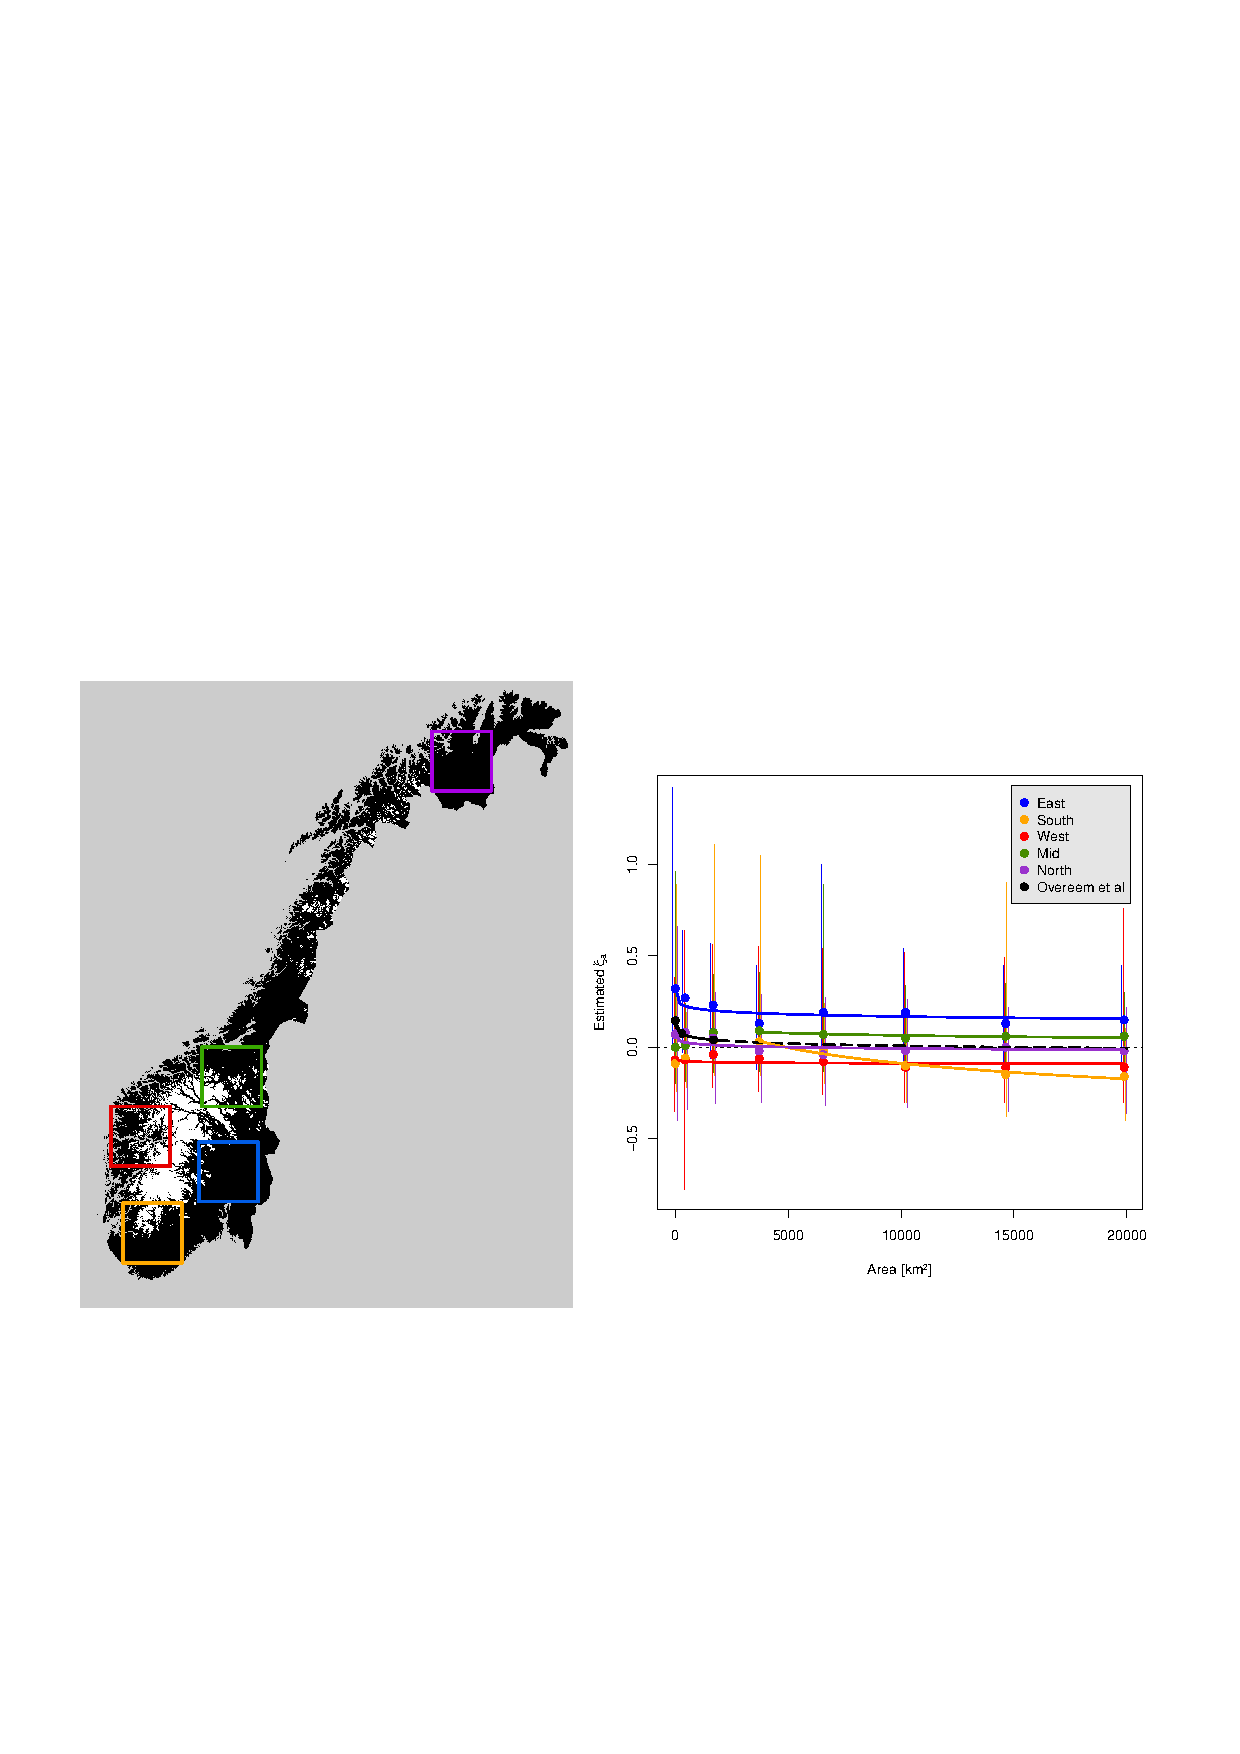
\includegraphics[width = 0.74\linewidth]{Figs/arealShape.pdf}
%\caption[shape]{\label{data:fig6}Left panel: Areas with topography in the background. Right panel: Estimated $\xi_{a}$ for the 5 regions and results from \cite{Overeemetal2010}, extended with a dashed curve.}
%\end{center}
%\end{figure}
We argued in the previous section that the range of extremes, and thus the $\xi_{p}$-parameter, varies according to dominating precipitation systems and orographic effects. Another aspect for areal precipitation is that different processes and degree of spatial correlation will create a different population of extremes depending on the size of the catchment.
For further analysis we selected 17 catchments in Norway, varying in size from 105 to 5693~$km^2$. The catchments were selected according to availability of SB-gf estimates and to represent different parts of the country. They are presented in Table~\ref{data:tab1} and in Fig.~\ref{data:fig6}.   

If the extremes converge towards a GEV Type I in larger areas, $\xi_{a}$ would be smaller than $\xi_{p}$ in areas where $\xi_{p}$ is positive, and vice versa. This is however not seen in Fig.~\ref{data:fig7}, where we plot the mean $\xi_{p}$ against $\xi_{a}$ in the catchments. But we note a small tendency to larger differences (deviation from the diagonal) in larger catchments.
%Reasons for this may include strong inhomogeneities in the Norwegian precipitation climate, the catchments being too small to see an effect, and also a possible misrepresentation of spatial correlation in the gridded dataset. 

To minimize the effects of inhomogeneity, we select two areas; Southeast and Southwest (cf. Fig.~\ref{data:fig2}) that are relatively homogeneous in terms of $\xi_{p}$. Positive $\xi_{p}$ values dominate the Southeast, while negative dominate the Southwest. Within the areas we select 25 points and estimate $\xi_{a}$ for increasingly larger areas around the points. Fig.~\ref{data:fig8} reveals a scale-break around 1500 $km^2$ in both areas, and a second scale-break around 6000 $km^2$ in the Southeast. These can probably be attributed to the geographical extent of different precipitation systems that produce extremes in the two areas, and confirm that we are dealing with a mixture of different extreme value distributions that complicates our study. The two scale-breaks in the Southeast indicate that a greater variety of precipitation types occur here, as suggested in Section 2.4, and that these precipitation types produce extremes from different distributions. After the last scale-break we note that $\xi_{a}$ decreases, reflecting the reduced spatial correlation as the area increases. In accordance with \cite{Overeemetal2010}, extremes converge from a GEV type II towards a GEV Type I distribution in the Southeast. In the Southwest, however, the Type III distribution is further strengthened. %This supports a hypothesis of the reduced spatial correlation being reflected as a lower $\xi_{a}$, regardless of $\xi_{p}$ being positive or negative, and undermine the alternative hypothesis of $\xi_{a}$ converging to zero in both cases. 
The latter may indicate that in areas of negative $\xi_{p}$ the assumptions for the central limit theorem, such as the observations being i.i.d., are not met. A reason for this might be that orographic enhancements have a non-linear and spatially intermittent effect, and hence contaminate the extreme value distribution. 
These findings have to be considered preliminary, and due to the strong gradients in the Norwegian precipitation climate along with possible misrepresentation of spatial correlation in the gridded dataset, a more thorough investigation of $\xi_{a}$ is necessary.   

\vspace{5mm}

\begin{table}[hbtp]
  \begin{tabular}{|l|c|c|c|c|}
    \hline
    \hline
    \textbf{Catchment} & \textbf{Size [$\mathbf{km^2}$] } & \textbf{Median elevation} & \textbf{PN [mm]} & \textbf{Reference} \\
	\hline
	1. Teksdal & 105/107 & 177 & 1300/1555 (+19.6\%) & \cite{Forland1997}\\
	\hline
	2. Lauvsnes & 114/107 & 209 & 1350/1380 (+2.2\%) & \cite{Isaksen2006}\\
	\hline
	3. Aursunda & 118/119 & 260 & 1300/1398 (+7.5\%) & \cite{Mamen2009}\\
	\hline
	4. Svartevatn & 210/204 & 1046 & 2050/2748 (+34.0\%) & \cite{Forland1991b} \\
	\hline
	5. Roskreppfjord & 282/266 & 1050 & 1450/1887 (+30.1\%) & \cite{Forland1991b}\\
	\hline
	6. Vekteren & 308/293 & 610 & 1250/1118 (-10.6\%) & \cite{Forland1991a}\\
	\hline
	7. Siljan & 490/492 & 220 & 1050/1157 (+10.2\%) & \cite{Forland1986b}\\
	\hline
	8. Aursj{\o}en & 487/496 & 1280 & 760/829 (+9.1\%) & \cite{Hanssen-Bauer1992}\\
	\hline
	9. J{\o}lstra & 570/573 & 680 & 2200/3130 (+42.3\%) & \cite{Forland1986a}\\
	\hline
	10. Namsvatn & 696/701 & 750 & 1300/1151 (+11.5\%) & \cite{Forland1991a}\\
	\hline
	11. Soneren & 701/754 & 540 & 900/989 (+9.9\%) & \cite{Hanssen-Bauer1991}\\
	\hline
	12. Sira & 1720/1554 & 693 & 2020/2529 (+25.2\%) & \cite{Forland1991b}\\
	\hline
	13. R{\o}ssvatn & 1500/1941 & 580 & 1200/1536 (+28.0\%) & \cite{Forland1988} \\
	\hline
	14. R{\o}ss{\aa}ga & 1800/1941 & 580 & 2000/1536 (-23.2\%) & \cite{Mamen2011b} \\
	\hline
	15. Barduelva & 2366/2107 & 671 & 575/892 (+55.1\%) & \cite{Forland1990b}\\
	\hline
	16. Arendal & 4200/4006 & 520 & 1150/1290 (+12.2\%) & \cite{Mamen2011a}\\
	\hline
	17. Virdnejavrre & 5693/5805 & 435 & 450/434 (-3.6\%) & \cite{Forland1994}\\
   \hline
   \hline
\end{tabular}
\caption[Areas]{\label{data:tab1}\sl Catchments sorted after increasing size. Median elevation is taken from the digital elevation model with 1 km resolution applied in the gridded dataset. PN is normal annual precipitation. For size and PN we show values used in SB-gf first, followed by values used in GB-GEV. The percentage difference between PN used in SB-gf and PN used in GB-GEV is given in parentheses.}
\end{table}

\clearpage

\begin{figure}[htbp]
\begin{center}
\includegraphics[width = \linewidth]{Figs/catchments_new.pdf} 
%\vspace{-15mm}
\caption[Map]{\label{data:fig6}Catchments and observation sites. Colored sites indicate long (>100 years) observational series separated into regions.}
\end{center}
\end{figure}

\begin{figure}[!htbp]
\begin{center}
\includegraphics[width = 0.65\linewidth]{Figs/shapeP_shapeA_new.pdf}
\caption[shape]{\label{data:fig7}Mean $\xi_{p}$ against $\xi_{a}$ in the catchments. The size of the dots indicates catchment size. The thick grey dashed line indicates the diagonal ($\xi_{a}$ = $\xi_{p}$) and the thin grey dashed lines indicate $\xi_{p}$ = 0 and $\xi_{a}$ = 0.}

\includegraphics[width = 0.65\linewidth]{Figs/shape_area.pdf}
\caption[shape]{\label{data:fig8}$\xi_{a}$, estimated from the gridded dataset, against area size in the Southeast (red) and the Southwest (blue) of Norway.}
\end{center}
\end{figure}

\clearpage

\subsection{GB-GEV}

Our analyses indicate a connection between relevant precipitation indices and the spatial distribution of the GEV $\xi$ parameter in Norway. We recognize, however, that further work is needed to present a model for $\xi_{a}$ according to empirical evidence. As a result, we here choose to estimate $\xi_{a}$ directly. The proposed method, GB-GEV, thus includes fitting the GEV distribution to annual maximum areal 24-hour precipitation extracted from the precipitation grid, using MLE to estimate the three GEV parameters. 

It is common practice to use PMP-estimates, which represent a precipitation amount with a return period of infinity, in the design of critical constructions like e.g. reservoir dams. %PMP is supposed to represent a precipitation amount with a return period of infinity. However, discussions in the literature point to great disagreement on whether there exists an upper limit to precipitation, and both ethical and technical issues are associated with the concept \citep{Benson1973,Koutsoyiannis2004a}. 
Great uncertainties are associated with the estimation of long return periods, and the evolvement of numerical weather (NWP) models introduces the possibility of perhaps more physically based PMP-estimates \citep{Cottonetal2003,WMO2009a}. With these considerations we have in this study not attempted a new statistical method for PMP-estimation, however, we suggest that a thorough analysis of NWP-based estimation methods is carried out in the future. 

\section{Method comparison and discussion}

We compare return level estimates from GB-GEV and SB-gf in the 17 catchments, making use of previously determined SB-gf estimates computed at MET Norway on different occasions (cf. Table.~\ref{data:tab1}). Percentage differences for M100, M500, and M1000 are shown in Fig.~\ref{data:fig9}. GB-GEV estimates lie within a 25\% deviation of SB-gf estimates in most catchments. In the wetter catchments where PN used in the two methods differ significantly, GB-GEV estimates are somewhat higher than SB-gf estimates, especially for M100 (see Fig.~\ref{data:fig10}). The largest deviation is seen in Svartevatn, where GB-GEV estimates are 40-60\% higher. A natural explanation for this is the elevation gradient for precipitation used in the gridded dataset, which in wet areas such as Svartevatn, is likely to generate serious overestimation since the elevation gradient is defined as a percentage. The growth factors in SB-gf seem to correspond to a somewhat higher positive $\xi_{a}$ compared to the estimated $\xi_{a}$ in GB-GEV. Consequently, in the case of GB-GEV > SB-gf for shorter return periods, the longer return periods might correspond quite well. While in the opposite case the difference will grow further with longer return periods. 

Figs.~\ref{data:fig11}-\ref{data:fig14} show examples of estimates from four catchments; Soneren, Siljan, Aursunda and Roskreppfjord, including empirical values. As these are grid-based empirical values, and thus biased towards GB-GEV, they can not be applied to determine the better model. The 95\% and 99\% confidence intervals, indicating the uncertainty in the GB-GEV estimates, are shown in the figures. It must be emphasized that this confidence interval only reflects the uncertainty in the estimation of the GEV parameters, while additional and unquantifiable uncertainty is associated with the gridded dataset. For longer return periods SB-gf stays within the confidence intervals of GB-GEV in all catchments, except at Sira where SB-gf moves slightly above the upper confidence level for M1000. 

Uncertainties in the gridded dataset are likely to influence our estimates, particularly in high-elevated and ungauged regions. Another aspect is the vertical precipitation gradient, known to overestimate precipitation in higher elevations. The latter, being defined as a percentage, produces an even greater overestimation of the extreme values. On the other hand, extremes in any interpolated dataset are often underestimated due to smoothing, and the relatively sparse station network results in many large precipitation events not being measured as small convective cells may travel between observation sites rather than across. In catchments located on the borders between different precipitation regimes, the spatial coherence might be reduced both due to the nature of different precipitation systems and the heterogeneous effect of the precipitation gradient. An important part of computing extreme areal precipitation estimates is to be aware of these effects and, while anticipating improved datasets, consider alternative estimation methods in the more uncertain regions.

A more comprehensive study of different precipitation types and their spatial distribution would be an interesting focus for future work. Numerical weather models or statistical pattern recognition \citep{Skaugen1997} can for instance be used to separate frontal from convective precipitation, which could further confirm the effect of precipitation types on the negative shape parameters seen in the Southwest. An analysis of the orographic effect on spatial correlation also remains a subject of future research.   

\begin{figure}[!htbp]
\begin{minipage}[t]{0.50\textwidth}
\centering
\includegraphics[width = \linewidth]{Figs/MT_perc_estShape.pdf}   %plot_retlev.R
\vspace{-5mm}
\caption[]{\label{data:fig9}Percentage difference in M100 (circle), M500 (triangle), and M1000 (square) between SB-gf and GB-GEV estimates. Grey background indicates catchments with large difference in PN used in the two methods.}
\end{minipage}
\hspace{10mm}
\begin{minipage}[t]{0.50\textwidth}
\centering
\includegraphics[width = \linewidth]{Figs/diffM100_diffPN.pdf}
\caption[]{\label{data:fig10}Percentage difference in M100 between SB-gf and GB-GEV estimates, against difference in PN used in the two methods. The grey solid line indicates the result of the linear regression, and the two grey dashed lines indicate no difference between the methods.}
\end{minipage}
\end{figure}

\begin{figure}[!htbp]
\begin{minipage}[t]{0.50\textwidth}
\centering
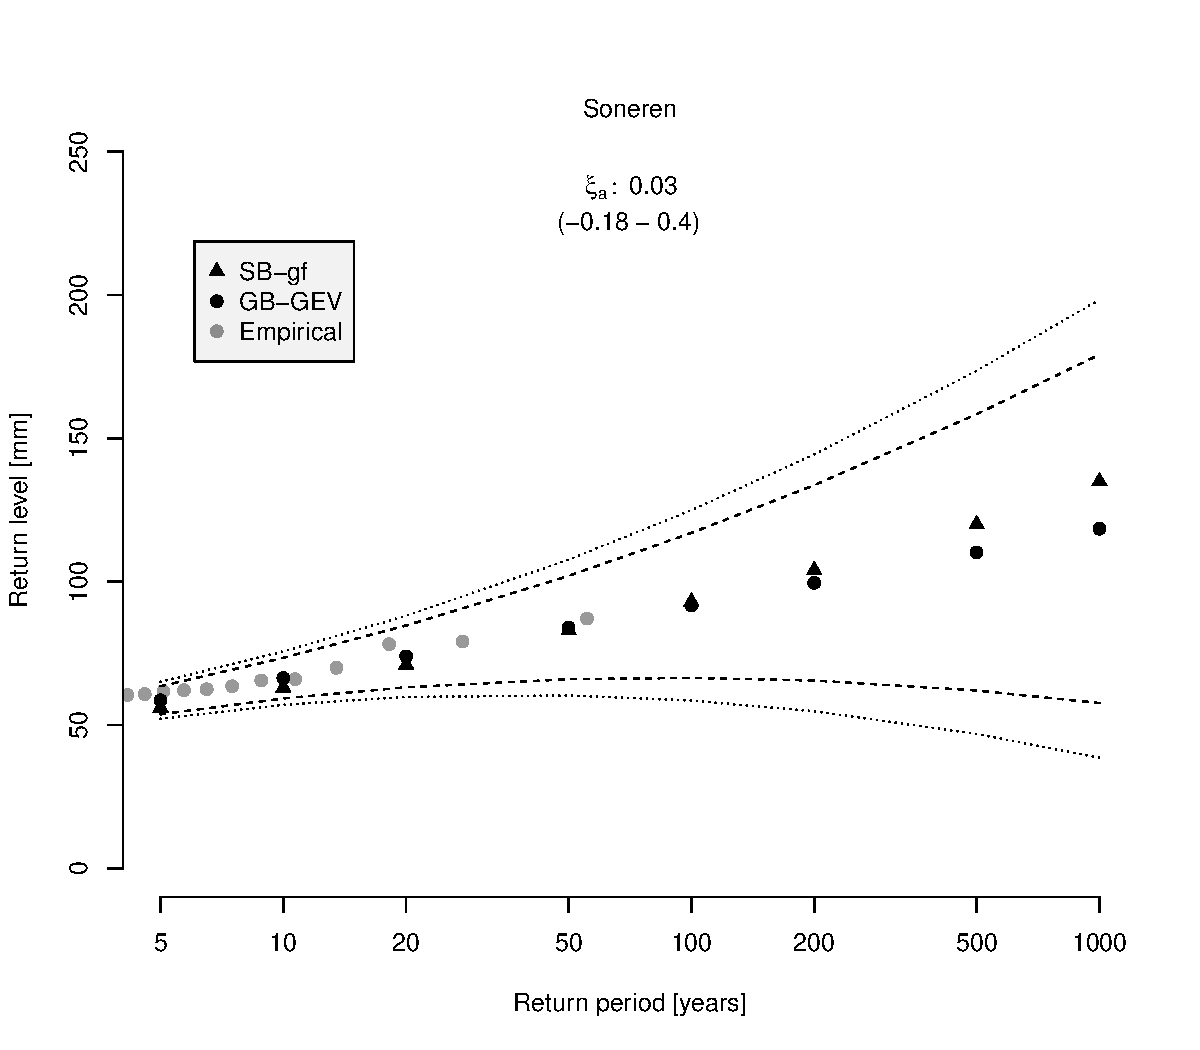
\includegraphics[width = \linewidth]{Figs/compareMT_Soneren.pdf}
\caption[]{\label{data:fig11}Estimated return levels for areal precipitation at Soneren catchment, using SB-gf and GB-GEV. Empirical values are from the gridded dataset. Dashed (dotted) line indicates the 95\% (99\%) confidence intervals.}
\end{minipage}
\hspace{10mm}
\begin{minipage}[t]{0.50\textwidth}
\centering
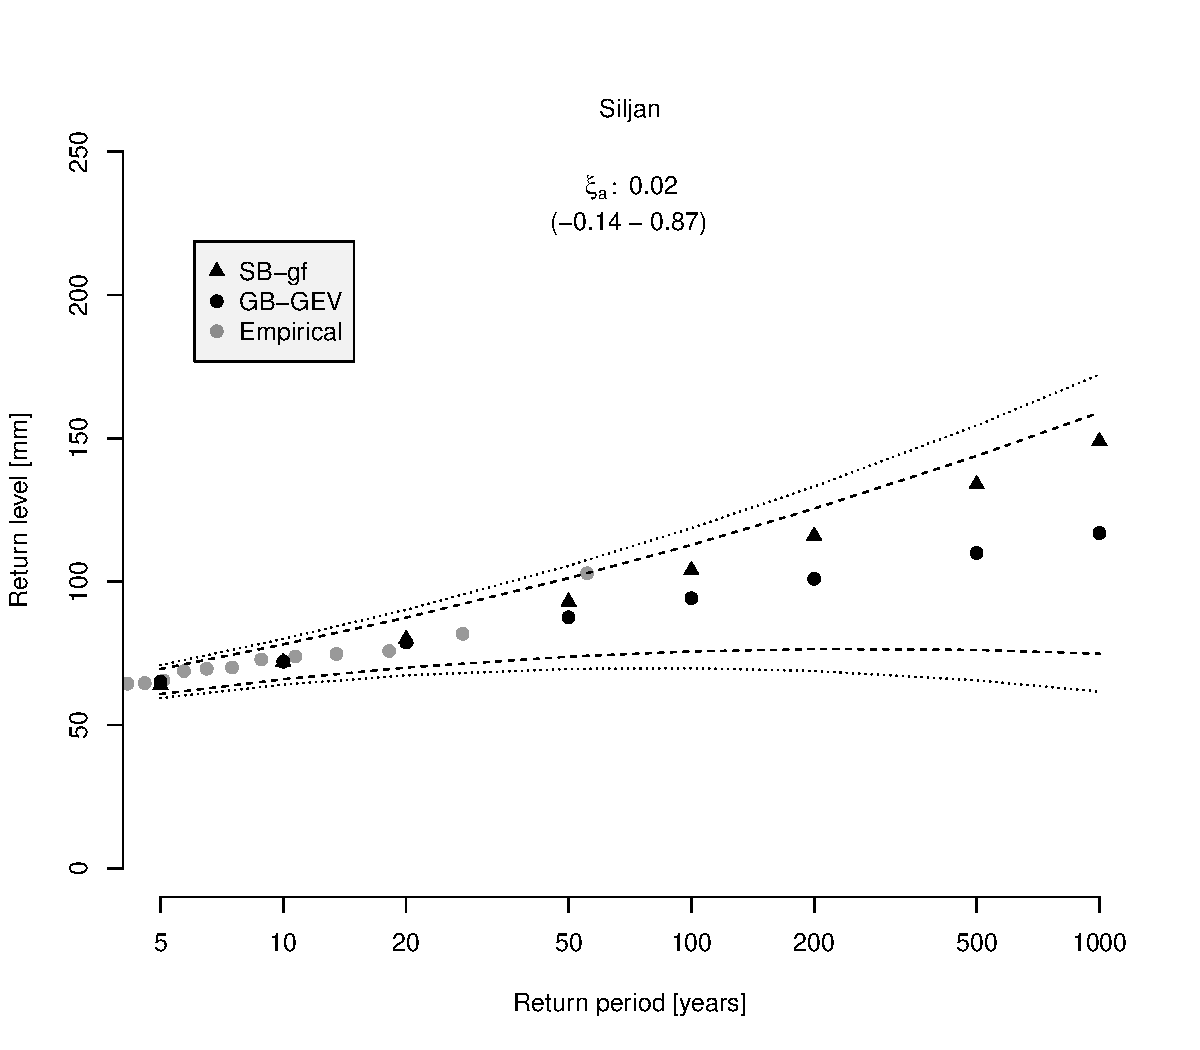
\includegraphics[width = \linewidth]{Figs/compareMT_Siljan.pdf}
\caption[]{\label{data:fig12}Same as Fig.\ref{data:fig10}, at Siljan catchment.}
\end{minipage}
\end{figure}

\begin{figure}[!htbp]
\begin{minipage}[t]{0.50\textwidth}
\centering
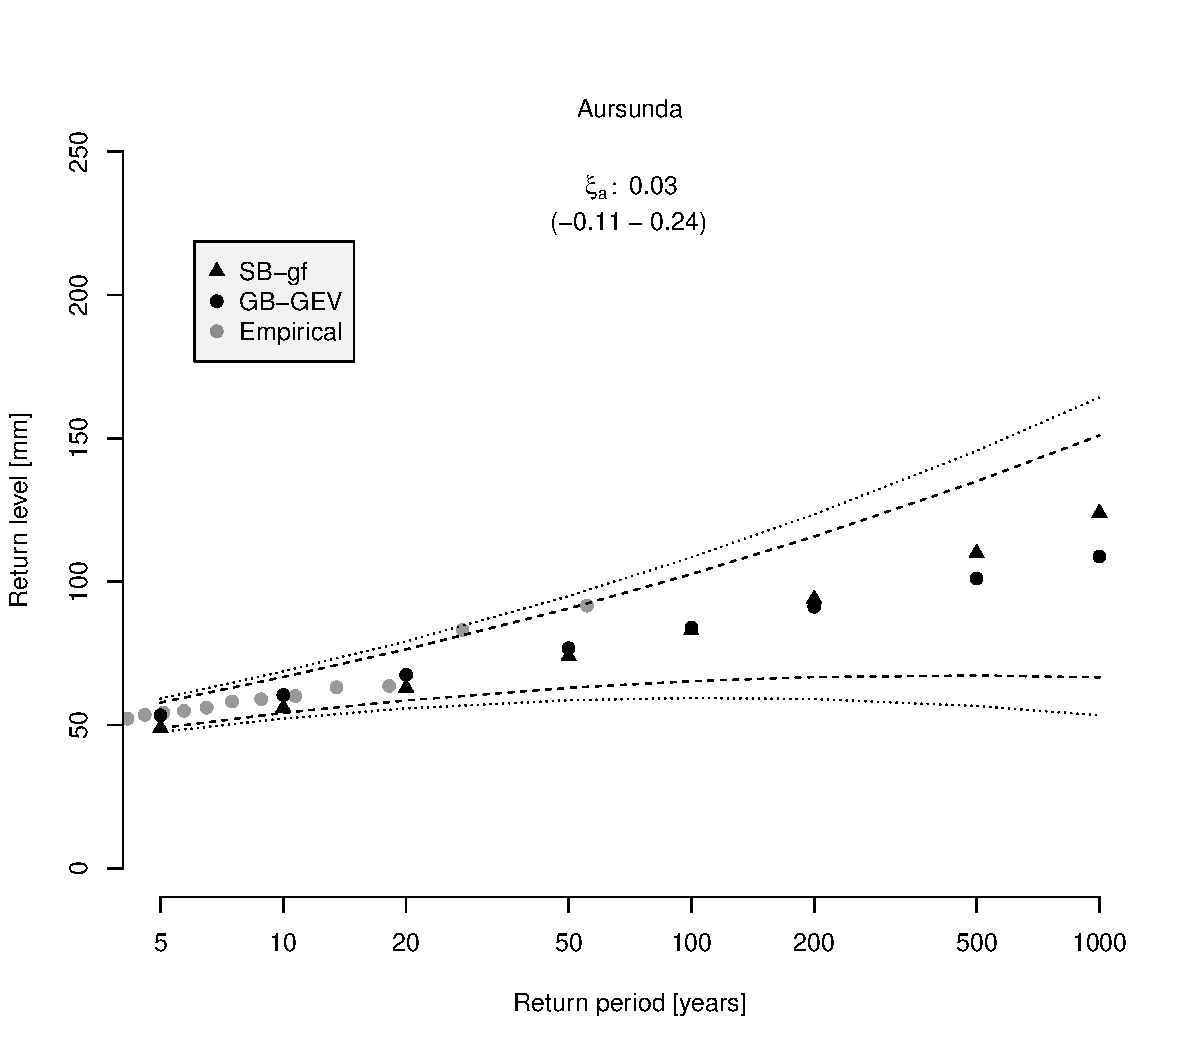
\includegraphics[width = \linewidth]{Figs/compareMT_Aursunda.pdf}
\caption[]{\label{data:fig13}Same as Fig.\ref{data:fig10}, at Aursunda catchment.}
\end{minipage}
\hspace{10mm}
\begin{minipage}[t]{0.50\textwidth}
\centering
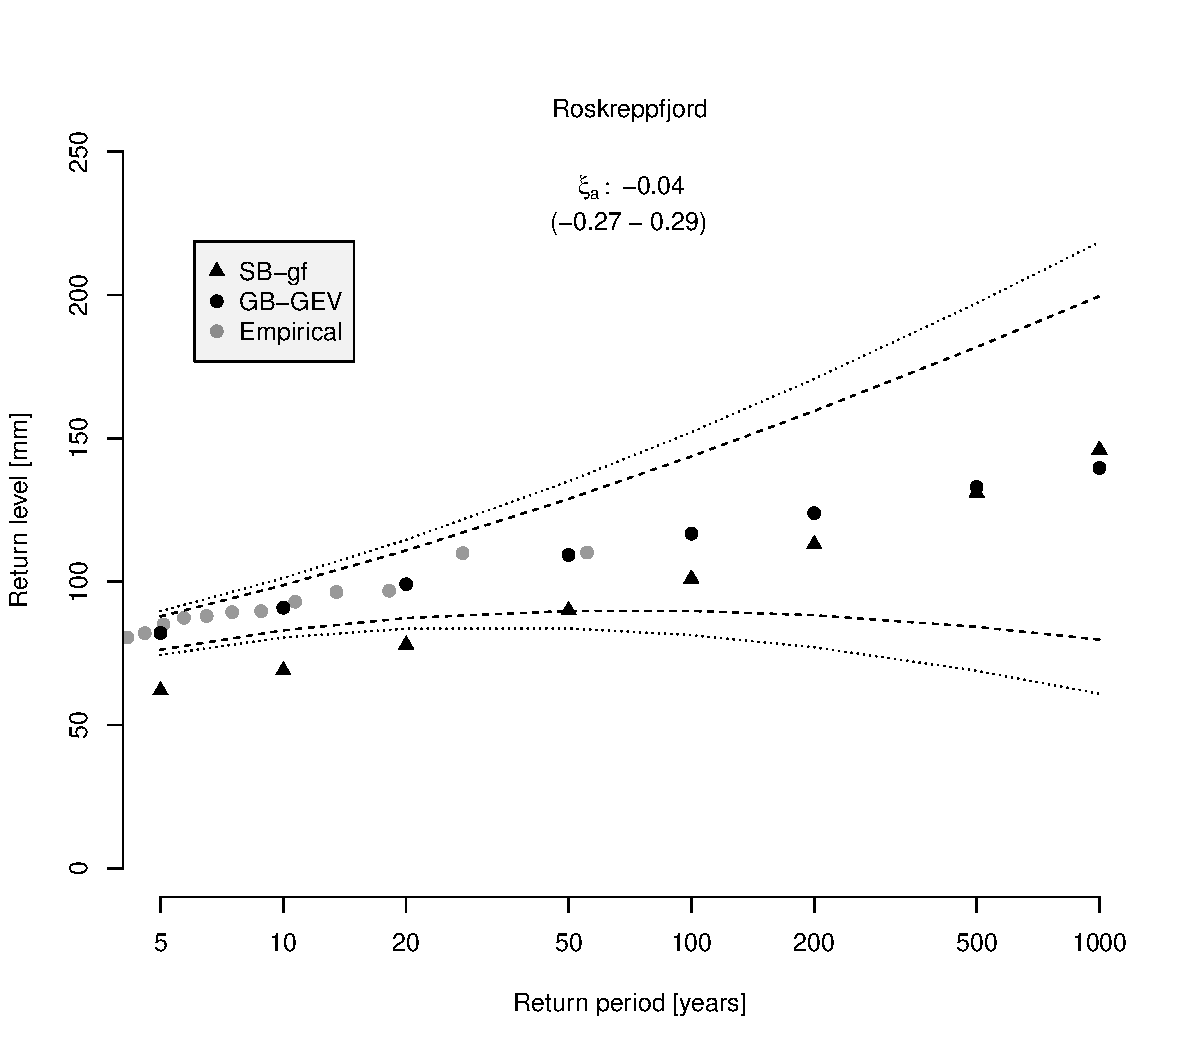
\includegraphics[width = \linewidth]{Figs/compareMT_Roskreppfjord.pdf}
\caption[]{\label{data:fig14}Same as Fig.\ref{data:fig10}, at Roskreppfjord catchment.}
\end{minipage}
\end{figure}

\clearpage


\section{Conclusions}

We propose a new grid-based method, GB-GEV, for estimating extreme areal precipitation in Norway. To the best of our knowledge we are the first to use fine-scale grids for this purpose, and to investigate the behavior of the GEV $\xi$ parameter in Norway. Estimates from GB-GEV are compared to estimates from the existing method at MET Norway, SB-gf. Due to large uncertainties and short time series, as well as the absence of areal precipitation measurements, it is difficult to indicate which estimates are better. However, there are relevant and decisive differences between the methods. Our findings can be summarized as follows:

\begin{itemize}
\item Grid-based methods are less manual and time-consuming compared to the station-based method, as well as more objective and consistent in terms of input data. In addition, estimates in ungauged catchments are easier to obtain. %Estimates are dependent on the quality of the gridded dataset, thus we emphasize the importance of its further development, such as dealing with the known issue of overestimation in high-elevated areas.

\item GB-GEV estimates are generally lower than SB-gf estimates, but lie within a 25\% deviation in most catchments.  

\item We have shown that $\xi_{p}$ varies spatially in Norway, seemingly depending on dominating precipitations systems and orographic enhancement. For areal extremes the catchment size plays an additional role due to the degree of spatial correlation. We also observe that record length influences the $\xi_{p}$-estimates and that the accuracy most likely increases with longer series. Our results suggest that $\xi_{a}$ should be modeled according to empirical evidence, however, a more extensive analysis and perhaps additional data sources are required before concluding on a suitable model.
\end{itemize}
 
\noindent The authors recognize that GB-GEV estimates are dependent on the quality of the gridded dataset. This means that estimates are less robust in areas with few observations and complex topography. Still, GB-GEV estimates will become more accurate as gridded products  improve in the future, and the suggested methodology provides more objective and geographically consistent results than the SB-gf method. GB-GEV can also be applied in estimating extreme precipitation from future climate projections. 


\section{Acknowledgement}

We thank the Norwegian Water Resources and Energy Directorate (NVE), Norwegian railway authority (Jernbaneverket) and Norwegian public roads administration (Statens vegvesen) for providing financial support to this study which is part of a PhD project. Valuable feedback from Torill Engen-Skaugen (MET Norway) and the two reviewers is appreciated.


\bibliography{/home/anitavd/Latex/anita}
\vspace{10mm}
\noindent*Available at http://met.no/Forskning/Publikasjoner/

\end{document}
